%%%%%%%%%%%%%%%%%%%%%%%%%%%%%%%%%%%%%%%%%%%%%%%%%
%%%%%%%%%%%% cap: vulnerabilities %%%%%%%%%%%%%%%%%
%%%%%%%%%%%%%%%%%%%%%%%%%%%%%%%%%%%%%%%%%%%%%%%%%

\chapter{Vulnerabilities}\label{cap:vulnerabilities}

\section{Brief history over vulnerabilities}

Ever since the very early days of internet (cca. 1990 \cite{curran2012rethinking}), the concept of vulnerabilities started becoming of greater interest to maliciously intended programmers. Simultaneously, the rise in the popularity of software made it such that vulnerabilities became harder to spot due to the more complex nature of programs. When putting together the above-mentioned, big amounts of people started attempting to exploit the nature of these vulnerabilities. 

\section{What is a vulnerability}\label{sect:whatisavulnerability}

A vulnerability is a weakness in either the code of a software or its configuration, which can allow the exploitation of it to different extents. They can be introduced unintentionally or unwarily, due to the lack of proper testing of the program before shipping. Chances exist that these vulnerabilities can also occur in different frameworks or libraries which may be used by the developers, therefore not being introduced by them; cases similar to the Log4J incident \cite{hiesgen2022race}. 

%Vulnerabilities are weaknesses or flaws in software code, design, or configuration that can be exploited by attackers to gain unauthorized access to a system, steal data, or cause system disruption. These vulnerabilities can be unintentionally introduced during the software development process, or they may exist in third-party components used in the software.

%With the advent of the internet, software vulnerabilities became an attractive target for hackers looking to gain access to valuable data or disrupt critical systems. One of the first high-profile instances of software vulnerabilities being exploited for malicious purposes was the Morris worm in 1988. This worm, created by a graduate student, exploited vulnerabilities in Unix-based systems to spread rapidly across the internet, causing significant disruption.

%Since then, vulnerabilities have been exploited in a wide range of attacks, from the infamous SQL Slammer worm in 2003 to the Equifax data breach in 2017. The frequency and severity of these attacks have led to increased focus on vulnerability management and software security. Today, organizations use a range of tools and techniques to identify and mitigate vulnerabilities in their software, including automated scanning tools, penetration testing, and code reviews.

\section{Risks of a vulnerability}

As priorly stated, vulnerabilities pose significant risks to companies behind the software, however, not just for them; individuals are at risk too. By abusing these factors, attackers can easily gain access to various kinds of information about every user. The types of information may vary from personal ones such as payment details and sensitive conversations to more public information, such as email addresses, names or birthdays. In a similar fashion, attackers can also exploit these scenarios to execute malicious code, cause system disruption or perform denial of service attacks. Similarly, data breaches are also often caused by these vulnerabilities.

\newpage
\section{Types of vulnerabilities}

With the risks covered, there are a handful of different types of vulnerabilities that can be exploited by attackers. These different types of vulnerabilities can be classified into various kinds, and we can put them as such:
\vspace{-2px}
\subsection{Different OS Vulnerabilities}
When it comes to different Operating Systems, they tend to differ at very low levels. A simple example of this would be big-endian address storing in comparison to little-endian address storing \cite{bradley2007defining} and a visual example can be seen below:
\begin{lstlisting}[caption = {Little-endian vs Big-endian}, columns=fixed, basewidth=0.5em, basicstyle={\ttfamily}, frame=lines, escapechar=!]
  Little-endian storing          ->           Big-endian storing
   0b10010011!\colorbox{light-gray}{11111000}!           ->           0b!\colorbox{light-gray}{11111000}!10010011
\end{lstlisting}









\vspace{-2px}
\subsection{Other Software Vulnerabilities}
Moving on in the hierarchy, we have what is known as "software vulnerabilities". These occur when there are flaws in the code of a software program that can be exploited by attackers. A few prime causes of it would be improper input validation, poor memory management, incomplete error handling, poorly designed 3rd party libraries, and lack of encryption.
\vspace{-2px}
\subsection{Configuration Vulnerabilities}
Configuration vulnerabilities on the other hand may not be as self-explanatory as the prior example. These kinds of risks refer to the configuration of software and more importantly, the system that is implicitly designed to act like the hosting device for the software or website in cause. The most common faults here would be weak passwords, misconfigured permissions or rights, unnecessary open ports, and finally, unpatched systems - which simply refer to systems that are not up to date with the latest security patches and updates.
\vspace{-2px}
\subsection{Physical Vulnerabilities}
While the concept of physical vulnerabilities not being in the main scope of this paper, together with the fact that attacks have started moving virtually for a very long time now, the concept of physical vulnerabilities is still not something to be overlooked. A few common ways that may result in leaks of information are theft of physical devices, physical access to data centers and social engineering - a type of attack that involves an individual posing as something they are not, to gain information out of the victim.
\vspace{-2px}
\subsection{Human Vulnerabilities}
Finally, a great factor in the process of data theft is the victims themselves. It is taken for granted that not everyone can excel at everything, and thus, some people have a harder time understanding the things they should be wary of, henceforth putting them at risk. Some of these factors are weak passwords, trusting unknown sources, lack of security awareness, and ultimately, being easily manipulated by others. 

\section{Notable attacks in recent years}

In the past years a variety of attacks had happened, those attacks varying from small scale to larger scale and the types of weaknesses abused varying from one to another. Below a few of the bigger-scale attacks within the past few years can be seen:


\begin{itemize}
    \item \textbf{Heartbleed} OpenSSL Vulnerability - \textit{2014} \cite{durumeric2014matter} \\
    Heartbleed is a vulnerability focusing on an error within an OpenSSL cryptographic software library that allowed the attackers to access the sensitive information of victims, among which passwords and private keys could be found too. 

    \item \textbf{Dirty COW} Security Vulnerability - \textit{2016} \cite{saleel2017linux} \\
    The Dirty COW incident was a security vulnerability that affected the Linux operating system kernel; it allowed attackers to gain write access to read-only memory mappings, including files that were supposed to be protected, essentially giving them root access.

    \item \textbf{LogPetya} Ransomware Attack - \textit{2017} \cite{aidan2017comprehensive} \\
    The Attack of LogPetya started with a Microsoft Windows vulnerability called Eternal Blue which allowed code to be executed on machines running Windows 7 or older alternatives. This opportunity was used to infect computers with a virus that encrypted the user's files and demanded ransom for their recovery.

    \item \textbf{Equifax} Data Breach - \textit{2017} \cite{berghel2017equifax} \\
    The Equifax Data Breach was a vulnerability found in the web application framework provided by Apache Struts, that allowed the attackers to ascertain the personal information of over 145 million customers.

    \item \textbf{BlueBorne} Bluetooth Vulnerability - \textit{2017} \cite{seri2019exploiting} \\
    As a way of linking devices, a Bluetooth vulnerability represents a great risk for the owners of any device that is capable of using it. The creators of BlueBorne made use of the vulnerability such that they will be able to take control of a device, spread malware, or steal private data without any user awareness or interaction.

    %\item \textbf{Wannacry} Ransomware Attack - \textit{2017} \cite{mohurle2017brief} \\
    %By abusing a vulnerability in Microsoft Windows, attackers were capable of spreading their ransomware all across the globe, disrupting a great number of businesses and organizations.

    \item Apache Web Server Vulnerability - \textit{2017} \cite{kim2017vuddy} \\
    Through the abuse of a buffer overflow vulnerability in the Apache Web Server, attackers could execute arbitrary code on the affected server and ultimately steal sensitive data of the users or even cause total system disruption.

    \item Cloudflare Leak - \textit{2017} \cite{baisakhiya2017cloud} \\
    Caused by a parsing bug in Cloudflare's edge servers, one website's data would inadvertently leak into another which gave the attackers access to passwords, cookies and encryption keys of websites using Cloudflare's services.

    
\end{itemize}

%Meltdown and Spectre (2018) - Vulnerabilities in computer processors that allowed attackers to steal sensitive information, such as passwords and encryption keys.

%In conclusion, vulnerabilities in software can pose significant risks to organizations and individuals, including data theft, malware attacks, DoS attacks, and account takeover. It is important for organizations to take proactive measures to identify and mitigate vulnerabilities in their software to minimize these risks.



\section{Testing for vulnerabilities}
When testing for vulnerabilities, it's best to keep in mind that no method is fail-proof and each method has its own drawbacks which may or may not be present in other alternatives. These methods can vary from human-based to machine-reliant and their methods may vastly differ from one another. The most commonly used methods are: \cite{al2013survey}

\begin{multicols}{2}
\begin{itemize}
    \item Code Reviews
    \item Fuzz Testing
    \item Risk Analysis
    \item Penetration Testing
    \item Compliance Testing
    \item Dynamic Testing
\end{itemize}
\end{multicols}

\subsection{Code Reviews}
Code reviewing is a manual process where a security analyst, if not the programmer, inspects the source code line by line in a linear pattern to identify any potential vulnerabilities that may pose a threat to the security of the software. As some older studies have concluded, this approach is the most time-consuming and arduous out of all others, as the person reviewing the code needs to have a deep understanding of the programming language together with the security risks that are associated with it \cite{ackerman1984software,fagan2002design}.

\subsection{Fuzz Testing}
Unlike the other types of tests and ways to analyze code, Fuzz testing (also known as Fuzzing) takes a less computational path and instead makes use of scripts to inject randomly generated data into the software. The type of input and data generated are typically nonsensical and follow no rules, except for the fact that they are used for one goal in particular (such as testing API requests for example). Given how Fuzzing is based on randomness, it is not guaranteed that it will detect all different types of issues, but it will help stabilize the software, API, or any other system in case upon receiving erroneous data. 

\subsection{Risk Analysis}
Risk analysis is the process of reviewing security requirements and identifying the risks based on the requirements; this is typically carried out during the design phase of the software and is done in correlation with an assessment of the likelihood and impact of the risk, therefore determining the importance of it \cite{khan2012systematic}. One frequently used technique is Failure Mode and Effects Analysis (or FMEA for short). This is a structured approach to also identifying and evaluating potential failures in the software to then take steps and minimalize, if not fully prevent, their effects \cite{lipol2011risk}. 

\subsection{Penetration Testing}
Also known as Ethical Hacking, Penetration Testing is the process of testing the Network Security of the system or server and whether or not the system resists attacks successfully, together with how it behaves when a vulnerability is exploited. Finally, it is also a common practice for "Ethical Hackers" to attempt to exploit vulnerabilities that have priorly been detected in previous review iterations \cite{caballero2007polyglot}.

\subsection{Compliance Testing}
A recent study from 2017 explains how roughly 40\% of breaches are due to employee carelessness \cite{balozian2017review} and according to another study, about 48\% of employees lack awareness in the security domain \cite{coopers2014global}. Given that information, Compliance testing has seen an increase in usage over the past couple of years. That being said, Compliance testing is the process that aims to ensure that the software systems tested are up to the standards of specific regulations, standards and guidelines. Similarly, they are typically also verified from a UML point of view \cite{bunyakiati2009compliance} and lately the concept of test and data-driven testing increasing \cite{steffens2018towards}.

\subsection{Dynamic Testing}
Conclusively, our last alternative, Dynamic Testing, is the opposite of Static Testing. This way of testing involves running the software and observing its behaviour in real-time in order to help identify errors that are difficult to detect through other means. This technique conjoins multiple other techniques such as penetration testing and fuzz testing in order to make the process as successful in detecting vulnerabilities as possible.

\section{Vulnerability detection through SCC}
When looking for vulnerabilities in the code of a software, it is important to remind ourselves about all factors that can influence a human's thought process during a review. These factors can include, but will not limit themselves to: Mood, bias for one's own work, time pressure, environment, etc. In contrast to that, tools are objective and will always function in the way they have been programmed to - or in other words, have no emotions nor a chance to miss a threat that it has been instructed to detect. On a similar note, one other important factor that should be taken into account is time conservation. A human will take time to analyze logically the flow of the code, whereas a program can perform the same task in a matter of moments, thus increasing performance.

\section{Testing criteria}
Granted the fact that vulnerabilities are caused by aspects that have not been taken into account, if not completely overlooked by humans, the difficulty in spotting these issues will be accounted for the final score of this category too.\smallskip\\  A group of programmers with different backgrounds has been asked to review the sample codes used to test the software on, where they will first be asked if they believe that there is a vulnerability in the code and secondly, if there is indeed a vulnerability, they will be asked to add a review of how difficult it would be to spot it. The ratings for each sample will be taken into account and an average of it will be made, together with a bias for the first answer. This will determine the difficulty of spotting the specific type of vulnerability and will be used as a side comparison for the results provided by the Static Code Analysis tools. 

\subsection{Types of tests}
Given the various types of vulnerabilities, the tests will be done on the following types of vulnerabilities:
\begin{multicols}{2}
\begin{itemize}
    \item SQL Injections
    \item Authentication
    \item Buffer Overflows
    \item Unclosed Files
    \item Poor memory management
    \item Insecure deserializing
    \item Server-Side Template Injection
    \item Insecure Direct Object References
    \item Session Hijacking
    \item Poor Hashing
    \item CSRF
    \item XSS
    \item Language-Specific vulnerabilities
\end{itemize}
\end{multicols}

\noindent The code snippets used for these tests have been written by hand and ultimately tested for vulnerabilities, assuring that there would be some way to abuse it. The programming languages that were used for the testing are C, C\#, PHP, and Python; the samples are able to be found on the GitHub repository referenced in \autoref{githubRef} 

\section{Tested Tools}
Due to conventional reasons, the tools that will be tested are going to require either a free variant or at least a trial. For the rest of the tools that will be used, we can enumerate:
\begin{multicols}{2}
    \begin{itemize}
        \item SonarQube
        \item Kodezi
        \item PVS-Studio
        \item Snyk Code
        \item Codiga
    \end{itemize}
\end{multicols}

\subsection{AI in Vulnerability Detection} \label{chatgpt}
With the rise in popularity of AI in the current days, researchers are now, starting to use AI to automatically generate much more elaborate rule sets for parsing code. For example, a team of researchers at ETH Zurich is now making a similar AI tool available for mainstream adoption. And granted this information, one of the most advanced and popular tools that is here to stay \cite{kasneci2023chatgpt}, ChatGPT, will also be used as a side comparison too in order to gain a better grasp over whether or not AI has a future in Static Code Analysis.

\section{Expectations}
Granted that both tools and humans have limitations and that AI is a permanently growing tool, it would not be a surprise if AI will outperform both humans and static code checkers in detecting vulnerabilities, and if not now then in the soon future. On the other hand, out of SCA tools and Humans, it would be expected having the tools be of a higher consistency. While humans can provide valuable insight and context, they can be prone to error and may also be limited by knowledge.

\vspace{-3mm}

\section{Results} \label{VSCAResults}

\subsection{Accuracy of Tools}

Following the template of the previous tool accuracy done in \ref{scaResults}, splitting will be done based on the type of languages that these vulnerabilities have been written in, this is done due to the fact that not all tools are capable of performing just as well on all languages. That being said, these language types are Low-Level languages (C \& C++), OOP languages (C\#), and finally, Scripting languages (Python \& PHP). Cutting to the chase, the average of tools for each category is:

\vspace{0.4cm}
\hrule    
\hspace{-0.6cm}
\begin{minipage}{0.5\textwidth}
\begin{figure}[H]
    \caption{Low-Level}
    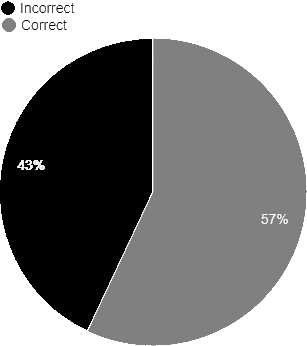
\includegraphics[scale=0.65]{./Images/VSCA low level.png}
\end{figure}
\end{minipage}
\hspace{0.8cm}
\begin{minipage}{0.45\textwidth}\raggedleft
\begin{figure}[H]
    \caption{OOP}
    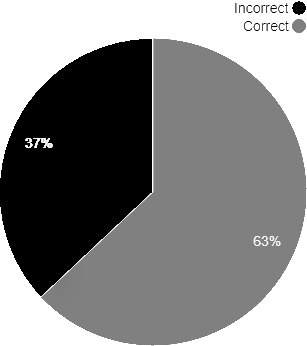
\includegraphics[scale=0.65]{./Images/VSCA OOP.png}
\end{figure}

\end{minipage}
\hspace{-0.6cm}
\begin{minipage}{0.5\textwidth}
\begin{figure}[H]
    \caption{Scripting}
    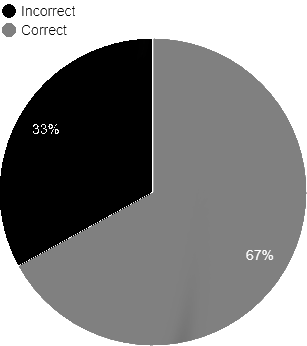
\includegraphics[scale=0.65]{./Images/VSCA scripting.png}
\end{figure}
\end{minipage}
\hspace{0.8cm}
\begin{minipage}{0.45\textwidth}\raggedleft
\begin{figure}[H]
    \caption{Median}
    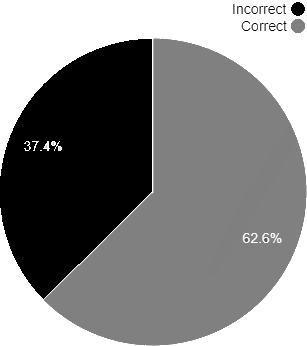
\includegraphics[scale=0.65]{./Images/VSCA avg.png}
\end{figure}

\end{minipage}
%\vspace{0.4cm}
%\hrule



\subsection{Accuracy of Humans}\label{humanacc}
\begin{center}
    With a total of 45 volunteers with different backgrounds and areas of expertise, below can be seen a graph representing their years of experience and their current field of work
\end{center}






\hrule    
\begin{figure}[H]
    \centering
    \caption{Volunteer Breakdown}
    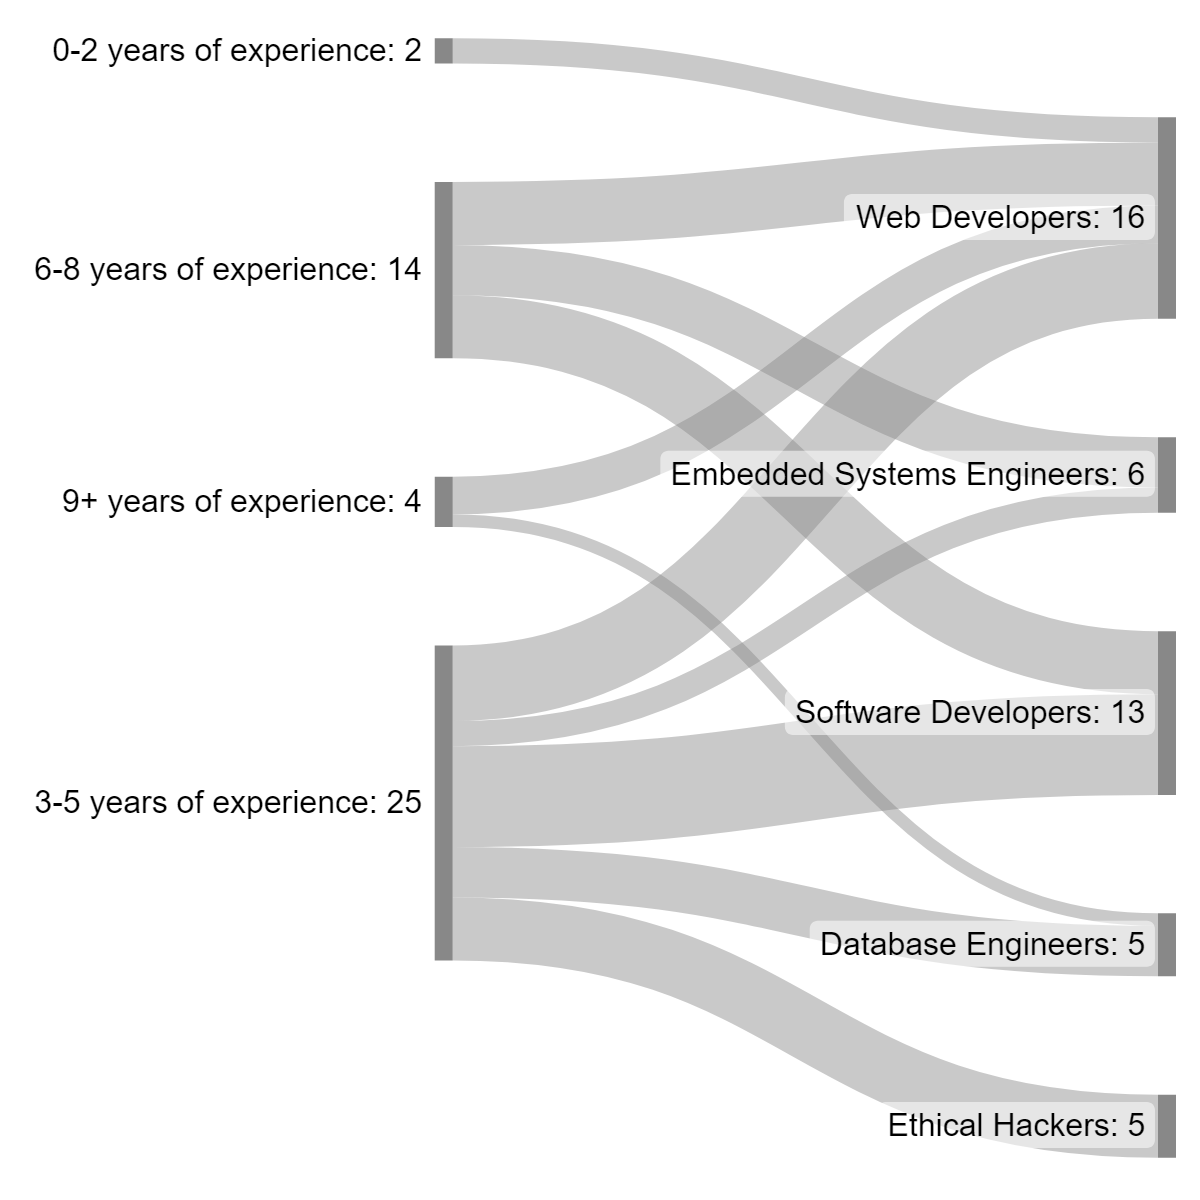
\includegraphics[scale=0.25]{./Images/breakdown.png}
\end{figure}
\hrule

\begin{center}
    And for a more detailed version of the volunteers' background and experience
\end{center}

\begin{lstlisting}[columns=fixed, basewidth=0.5em, basicstyle={\ttfamily},nolol]
Embedded Systems Engineers:             
                3-5 years - 2           Web Developers:
                6-8 years - 4                     0-2 years - 2
                                                  3-5 years - 6
   Database Engineers:                            6-8 years - 5
                3-5 years - 4                     9+  years - 3
                9+  years - 1                   
                                            
    Software Developers:                 Ethical Hackers:
                3-5 years - 8                     3-5 years - 5
                6-8 years - 5

\end{lstlisting}
\vspace{0.3cm}
\noindent The form the volunteers had to fill out provided them with 32 code snippets and asked them if there is a vulnerability present in the particular snippet. If they believe there is a vulnerability, they will then be asked to rate the difficulty of an average programmer with similar knowledge to theirs spotting the vulnerability. This rating was on a scale of 0 to 5 where 0 would be equivalent to "an obvious vulnerability" and 5 being something that will probably go under the radar, at least according to the opinion of the form-filler. In order to simplify the results, the ratings ranging from 0 to 2 will be treated as "easy to spot" and from 3 to 5 as "difficult to spot".\\

\noindent Primarily, there were 3 main types of vulnerabilities that the volunteers had to spot, each being split into multiple forms of it and in different languages. These 3 types are Back-end vulnerabilities (XSS, CSRF, Unrestricted file uploads, etc.), Overflows(Memory, Pointers, etc.), and Improper Sanitizing (SQL Injections, Paths, Direct object references, etc). For each category, a chart will be provided with the average accuracy of the volunteers and conclusively, one last for the overall standings of all categories.

\vspace{0.4cm}
\hrule    
\hspace{-0.6cm}
\begin{minipage}{0.5\textwidth}
\begin{figure}[H]
    \caption{Back-end}
    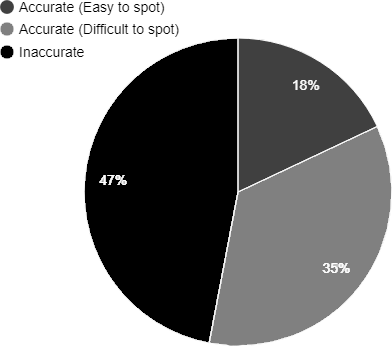
\includegraphics[scale=0.65]{./Images/web.png}
\end{figure}
\end{minipage}
\hspace{0.8cm}
\begin{minipage}{0.45\textwidth}\raggedleft
\begin{figure}[H]
    \caption{Sanitizing}
    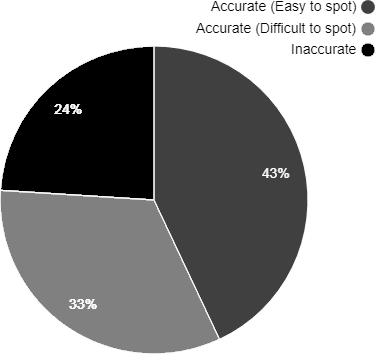
\includegraphics[scale=0.65]{./Images/unsanitized.png}
\end{figure}

\end{minipage}
\hspace{-0.6cm}
\begin{minipage}{0.5\textwidth}
\begin{figure}[H]
    \caption{Overflows}
    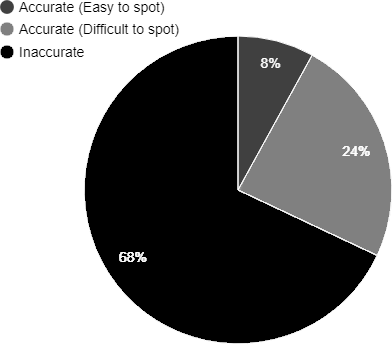
\includegraphics[scale=0.65]{./Images/overflows.png}
\end{figure}
\end{minipage}
\hspace{0.8cm}
\begin{minipage}{0.45\textwidth}\raggedleft
\begin{figure}[H]
    \caption{Median}
    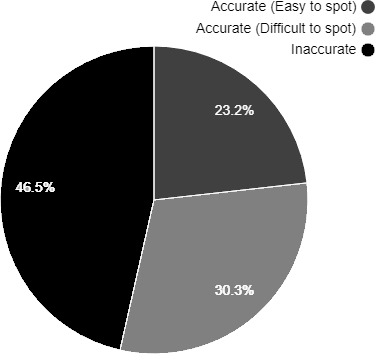
\includegraphics[scale=0.65]{./Images/avg.png}
\end{figure}

\end{minipage}
\vspace{0.4cm}
\hrule

\noindent As can be seen, on average, approximately half of the vulnerabilities went undetected by our volunteers. One thing worth mentioning is how the form presented code snippets of at most 30 lines of code, henceforth, the bias towards overlooking a possible vulnerability should go up when comparing these to production code.

% \hrule
% \vspace{-0.8cm}
% \begin{minipage}{0.58\textwidth}
% \begin{figure}[H]
%     \centering
%     \caption{Static Code Review Cycle}
%     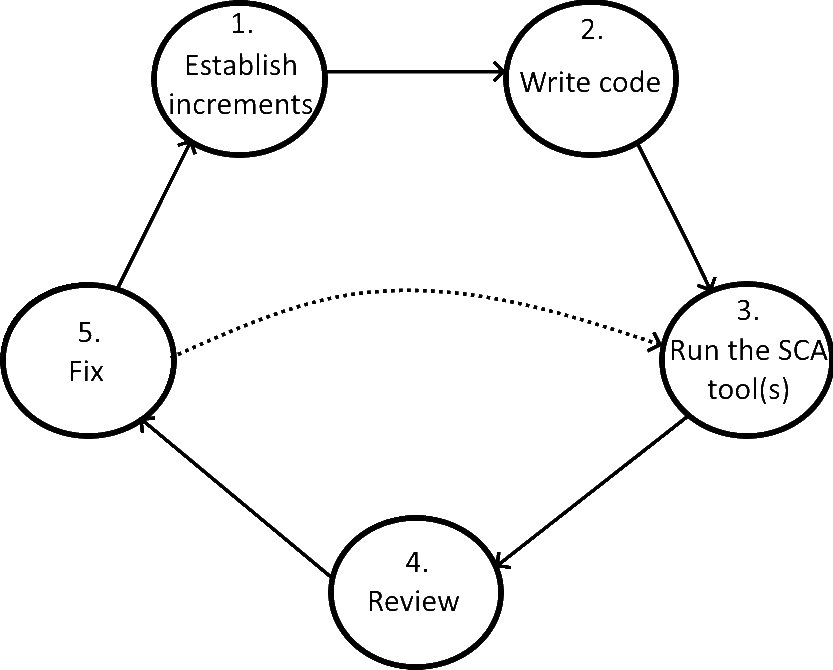
\includegraphics[scale=0.4]{./Images/sca2.png}
% \end{figure}
% \end{minipage}
% \begin{minipage}{0.40\textwidth}\raggedleft
% \vspace{1.5cm}
% \begin{figure}[H]
%     \centering
%     \caption{Static Code Review Cycle}
%     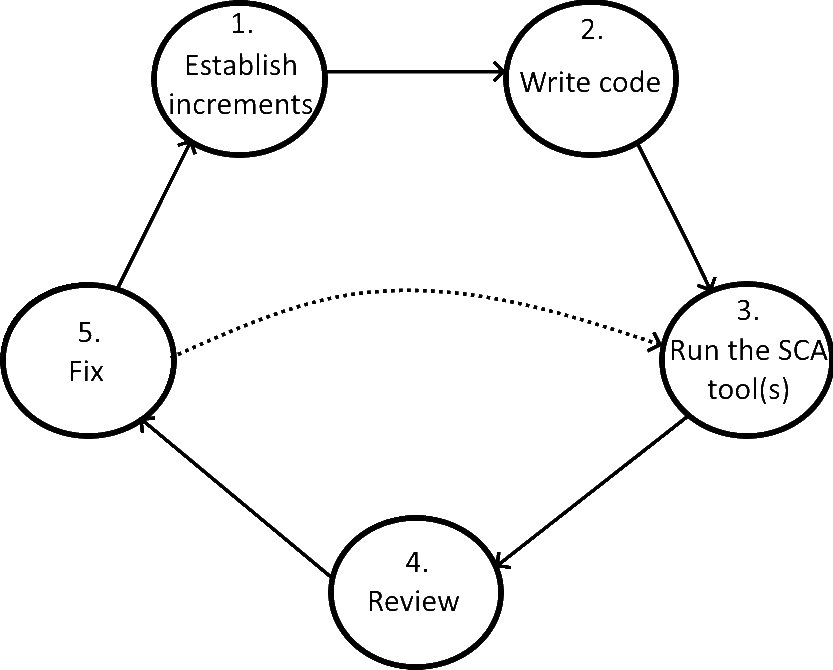
\includegraphics[scale=0.4]{./Images/sca2.png}
% \end{figure}
% \end{minipage}
% \vspace{0.3cm}
% \hrule



% 3-5 years of experience [6] Web Developers
% 6-8 years of experience [5] Web Developers
% 9+ years of experience [3] Web Developers
% 0-2 years of experience [2] Web Developers

% 3-5 years of experience [8] Software Developers
% 6-8 years of experience [5] Software Developers

% 6-8 years of experience [4] Embedded Systems Engineers
% 3-5 years of experience [2] Embedded Systems Engineers

% 3-5 years of experience [5] Ethical Hackers

% 3-5 years of experience [4] Database Engineers
% 9+ years of experience [1] Database Engineers
    
\subsection{Accuracy of AI}

As a last test in detecting vulnerabilities, ChatGPT has been asked to determine whether the code snippets provided to the responders from \ref{humanacc} contain any form of vulnerabilities, and if they do, to provide the name and solution. Upon multiple similar prompts, it became quite clear that was no consistency between the provided answers. Sometimes completely functional code would be deemed vulnerable due to too much memory management and sometimes vulnerable code would either be considered safe or as unsafe due to completely unrelated reasons, therefore making AI a very unstable resource/alternative.\\

\noindent Disregarding the above however, below can be seen the accuracy of ChatGPT in detecting the same vulnerabilities as the volunteers from the previous point after being provided a list of all possible vulnerabilities that may be encountered in the prompted code snippets. \\

\noindent\textbf{Disclaimer:} The percentages shown below may fluctuate for subsequent attempts.

%64.28\%  - 2x "partly correct" 
% C - buffer overflow: correct
% C - no file close: 			incorrect
% C - no free:                            incorrect
% C - ScanF: correct

% C# - Deserealize: partly correct
% C# - unsafe: correct
% C# - IDOR: correct
% C# - integer overflow: partly correct
% C# - integer overflow2: correct
% C# - SSTI:                               incorrect
% C# - SQL: correct
% C# - URaF: correct

% PHP - eval: correct
% PHP - include: correct
% PHP - Session Hijacking: correct
% PHP - unserialize: correct
% PHP - variable:                        	  incorrect

% PY - Bad error handling:  		  incorrect
% PY - Bad Hash: correct
% PY - BAaSM: 				  incorrect
% PY - CSRF: correct
% PY - Information leakage: correct
% PY - OS command injection: correct
% PY - Overflow: correct
% PY - Path:                		  incorrect
% PY - SQL: correct
% PY - Unrestricted file upload: 		  incorrect
% PY - XSS: 				  incorrect

% 64.28\% correct

\begin{figure}[H]
    \caption{ChatGPT Accuracy}
    \label{chatgptaccuracy}
    \centering
    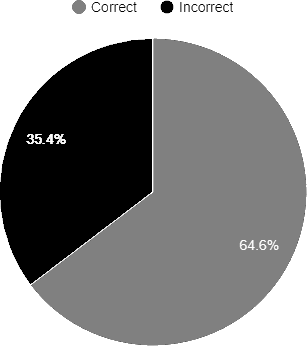
\includegraphics[scale=0.75]{./Images/chatGPT.png}
\end{figure}

\newpage
\subsection{Final Results} 

\hrule
\begin{minipage}{0.5\textwidth}
\begin{figure}[H]
    \caption{Tools}
    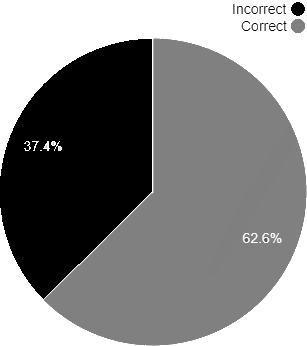
\includegraphics[scale=0.75]{./Images/VSCA avg.png}
\end{figure}
\end{minipage}
\hspace{0.8cm}
\begin{minipage}{0.45\textwidth}\raggedleft
\begin{figure}[H]
    \caption{Humans}
    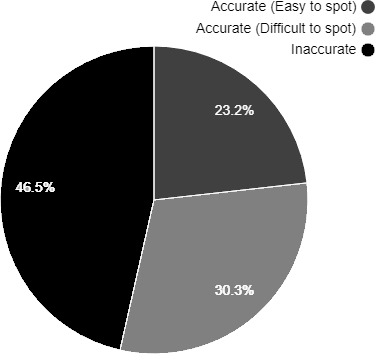
\includegraphics[scale=0.75]{./Images/avg.png}
\end{figure}

\end{minipage}
\vspace{0.4cm}
% \begin{figure}[H]
%     \caption{AI}
%     \centering
%     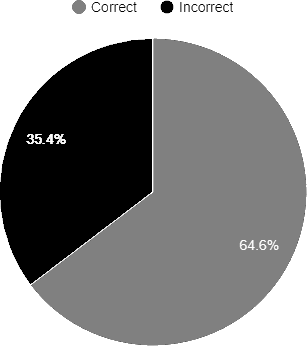
\includegraphics[scale=0.75]{./Images/chatGPT.png}
% \end{figure}
\hrule
\vspace{0.4cm}

\noindent Conclusively, in the comparison between the three for detecting vulnerabilities in code, it was found that Tools outperformed humans for smaller code snippets.
%AI was the most accurate with a success rate of 64.28\%, followed by SCA tools with a 57.85\% success rate, and lastly, humans, with a 53.5\% success rate.
While humans have a better understanding of the context and theoretical intent of the code, they are prone to making mistakes and thus this percentage may fluctuate greatly, in both directions. Tools are useful for automating repetitive tasks and can detect known patterns of errors, however, they may not be able to identify more subtle issues all the time and as such, while they seemingly outperformed the competition, they should she used as a helper rather than a guide.\\

%\subsubsection{Is AI proving itself worthy?}

\noindent And to answer the question that was opened in \ref{chatgpt}, given the results shown in Figure \ref{chatgptaccuracy}, AI has great potential in the future and if approached properly, could possibly be integrated into different SCA tools in order to drastically improve their performance and utility.